\tolerance=1600
\chapter{Navržená hra - Asteroidy}
V této úvodní kapitole se seznámíme se základním chováním a cílem hry. 
Vysvětlíme zde základní zákonitosti, jaké objekty se ve hře vysktují, jaký mají význam a jak s nimi manipulovat.

\section{Herní logika}
Asteroidy jsou hra pro dva hráče. 
Každý z hráčů ovládá svou vesmírnou loď.
Prostředí hry má představovat zjednodušený vesmírný prostor, kde neplatí gravitační ani odporové síly.
To má tedy za následek, že když se vesmírná loď rozletí v nějakém směru, tak v tomto směru letí i nadále i bez dalšího akcelerování.
\par
\label{HraniceProsotru}
Vesmírný prostor je v této hře nekonečný a dalo by se říct jistým způsobem cyklický, pokud vesmírná loď proletí dolní hranicí herního prostoru, tak nezmizí, ani nenabourá, ale objeví se na stejné pozici jen na horní hranici a opačně. Analogicky to platí i s bočními hranicemi.
Vesmírné lodě sebou mohou prolétávat a nedochází ke srážce.
Nejsou zde žádné statické překážky, kterým by bylo třeba se vyhnout. Co ale může způsobit srážku s vesmírnou lodí jsou asteroidy.    
\par
Asteroidy se generují na náhodných místech a s náhodným směrem i rychlostí letu. Nové asteroidy během hry vznikají tím častěji, čím déle hra trvá.
V boji s asteroidy má hráč v zásadě dvě možnosti. Buď se může pokusit danému asteroidu vyhnout, tím že s lodí pohne mimo trajektorii asteroidu, anebo může asteroid sestřelit.
Každý hráč má omezený počet životů a každá srážka lodě s asteroidem ubere hráči část jeho životů.
\par
Hráč má k dispozici dva typy střel, obyčejnou a rozdvojovací. Vystřelená střela má značně vyšší rychlost než vesmírné lodě i než kolem letící asteroidy.
Střely nejsou primárně určeny k přímému zasažení lodě protihráče, vesmírné lodě jsou k nepřátelským střelám imunní.
Smyslem střel je sestřelování letících asteroidů, pomocí kterých teprve může k zásahu nepřítele dojít. Asteroidy mohou mít tři velikosti. Náhodně vytvořený asteroid je vždy největší. Každým rozstřelením asteroidu vznikají asteroidy o stupeň menší velikosti.
Nově vytvořené asteroidy vznikají na základě typu rozstřelení na místě původního sestřeleného asteroidu. Typ rozstřelení závisí na druhu střely, jakou byl asteroid sestřelen. 
\par
V případě střely obyčejné vznikne namísto původního asteroidu jeden menší, který letí stejným směrem jako střela, která ho zasáhla.
V případě střely rozdvojovací se původní asteroid rozstřelí na dva menší, kde každý z nich je oproti směru střely vychýlen o 15\textdegree\ po a proti směru hodinových ručiček.
Pokud je zasažen asteroid nejmenší velikosti, tak již žádné další asteroidy nevznikají. 
Rychlost asteroidů je nepřímo závislá na jejich velikosti, čím je asteroid menší, tím vyšší rychlost má.
\par
Asteroidy vzniklé rozstřelením se v jistém pojetí stávají projektily daného hráče, přičemž hráč nemůže být zasažen takto vytvořenými vlastními projektily.




\section{Cíl hry}
Během hry vzniká postupně více a více asteroidů, čímž je postupně stále obtížnější se všem vyhýbat, nebo je sestřelit.
Hráč nemůže zranit nepřítele střelou přímo, může se ale snažit rozstřelit nějaký z kolem letících asteroidů tak, aby pomocí nově vzniklých asteroidů zasáhl nepřítele.
Cílem hráče je ovládat svou loď takovým způsobem, aby nepříteli došly životy dříve než jemu samému. Hra končí pokud libovolnému z hráčů dojdou životy, v takovém případě se druhý hráč stává vítězem.

\begin{figure}[H]

    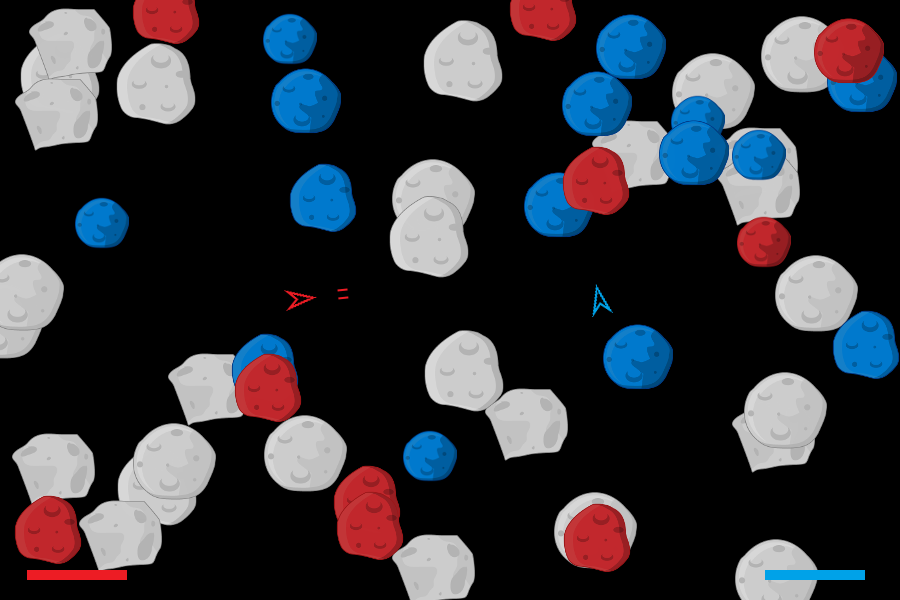
\includegraphics[width=145mm, height=100mm]{./Obrazky/UkazkaHry.png}
    \caption{Screenshot ze hry}
    \label{obr01:}
    \end{figure}